\documentclass[tikz,border=10pt]{standalone}
\usepackage{tikz}
\usetikzlibrary{calc, angles, quotes}

\begin{document}
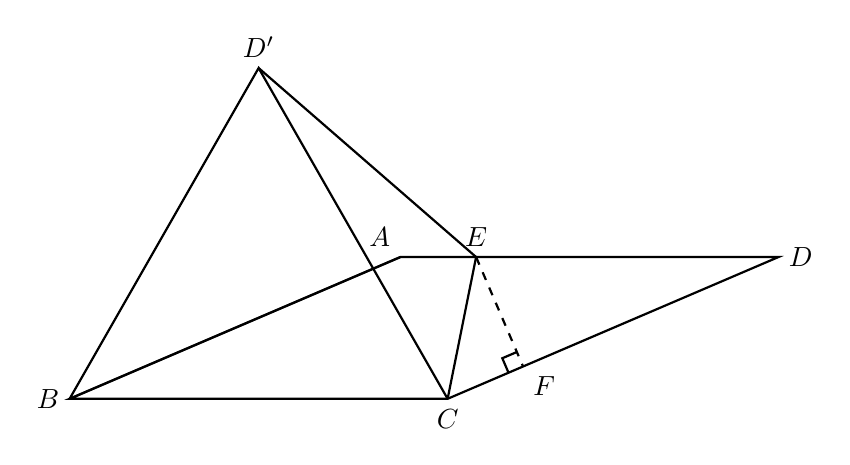
\begin{tikzpicture}[>=stealth, thick, scale=1.2]

    % --- 1. 定义核心顶点 (基于平行四边形视角) ---
    % 设定 B 为原点，C 在 x 轴上
    \coordinate (B) at (0,0);
    \coordinate (C) at (4,0);
    \coordinate (A) at (3.5,1.5);
    \coordinate (D) at ($(A)+(C)-(B)$); % 平行四边形顶点 D: D = A + C - B

    % --- 2. 定义折叠/特殊点 ---
    % D' 是折叠后的顶点位置
    \coordinate (D_prime) at (2,3.5);
    % E 是 AD 上的一点
    \coordinate (E) at ($(A)!0.2!(D)$);
    % F 是 CD 上的一点，EF 垂直于 CD (投影点)
    % 使用 TikZ 的 projection 计算 F 点
    \coordinate (F) at ($(C)!(E)!(D)$);

    % --- 3. 绘制实线路径 (可见轮廓) ---
    \draw (B) -- (C) -- (D) -- (A) -- cycle; % 原始平行四边形底座轮廓
    \draw (B) -- (D_prime) -- (C);           % 折叠后的侧面三角形
    \draw (D_prime) -- (E);                  % 连接 D' 到 AD 上的 E 点
    \draw (C) -- (E);                        % 连接 C 到 E 点

    % --- 4. 绘制虚线 (辅助线/不可见线) ---
    \draw[dashed] (E) -- (F);                % 垂线 EF
    \draw (B) -- (A);                        % BA 实际上部分被遮挡或作为背景

    % --- 5. 绘制直角标记 ---
    % 标注 EF 垂直于 CD
    \pic [draw, angle radius=2mm] {right angle = E--F--C};

    % --- 6. 标注文本标签 ---
    \node[left] at (B) {$B$};
    \node[below] at (C) {$C$};
    \node[right] at (D) {$D$};
    \node[above left] at (A) {$A$};
    \node[above] at (D_prime) {$D'$};
    \node[above] at (E) {$E$};
    \node[below right] at (F) {$F$};

\end{tikzpicture}
\end{document}